\documentclass{article}

\usepackage{polski}
\usepackage[utf8]{inputenc}
\usepackage{booktabs}
\usepackage{biblatex}
\usepackage{pdfpages}

\usepackage{graphicx}
\usepackage{float}
\usepackage{geometry}
\usepackage{listings}
\geometry{
	a4paper,
	total={170mm,257mm},
	left=35mm,
	right=35mm,
	top=35mm,
	bottom = 25mm
}
\usepackage{etoolbox}
\patchcmd{\thebibliography}{\section*{\refname}}{}{}{}
  

\begin{document}	

\includepdf[pages={1}]{strona-tytulowa.pdf}
\tableofcontents

\newpage
	
\listoffigures
\newpage

\listoftables	
\newpage

	
	
\section{Wstęp}
	\subsection{Cel projektu}
		Celem projektu jest zbadanie wpływu zmiany ilości wątków na czas działania programów.
	\subsection {Zakres projektu}
	Projekt obejmuje implementację oraz zbadanie czasu działania algorytmów grafowych poszukiwania najkrótszej ścieżki pomiędzy wszystkimi wierzchołkami. Problem znany jest powszechnie jako problem komiwojażera.
\section{Sformułowanie problemu}
		Problem komiwojażera jest problemem optymalizacyjnym, polegającym na znalezieniu ścieżki pomiędzy ustalonymi miastami dla następujących warunków: 
		\begin{itemize}
			\item wszystkie miasta są odwiedzone dokładnie jeden raz
			\item rozpoczynamy i kończymy w tym samym mieście.
			\item koszt (suma wag krawędzi) jest najmniejszy z wszystkich możliwych
		\end{itemize}
		Oznacza to, że należy znaleźć taki cykl Hamiltona dla grafu reprezentującego zbiór miast, dla którego suma wag wybranych krawędzi jest najmniejsza.
		
	\subsection{Opis wariantów rozwiązywania problemu}	
		\subsubsection{Przegląd zupełny}
				W algorytmie przeglądu zupełnego zastosowana jest taktyka brutalna, silna. Systematycznie sprawdzane są kolejne wartości funkcji długości drogi dla wszystkich możliwych permutacji wierzchołków. Zastosowany algorytm w sposób sprytny i zwinny, poprzez rekurencję zapewnia sprawdzenie wszystkich możliwości.
		\subsubsection{Branch\&Bound}
			
				W rozwiązaniu powyższego problemu zastosowano metodę podziału i ograniczeń. Metoda ta jest metodą optymalizacji dyskretnej, opierając się na podejściu \textit{dziel i zwyciężaj}.
				W każdym kroku algorytmu przeglądane jest drzewo potencjalnych rozwiązań. Jeżeli natrafimy na węzeł, który jest liściem, czyli można określić dla niego długość drogi komiwojażera, sprawdzamy, czy nowo znaleziona wartość nie jest lepsza od aktualnie zapisanej. Jeżeli tak jest, to zapamiętujemy nowe rozwiązanie. W przypadku, gdy dany węzeł nie jest liściem, tworzymy dla niego pod-problemy. W tym celu odwiedzamy kolejne miasto starając się oszacować dolne ograniczenie kosztów całej trasy. W tym projekcie wykorzystano najprostszy sposób szacowania. Na początku z macierzy sąsiedztwa wycinana jest przekątna, następnie kolumny i wiersze miejsc już odwiedzonych. Następnie wartości z tak przygotowanej macierzy są sortowane w kolejności niemalejącej. Szacowanie polega na dodaniu do siebie tylu kolejnych wartości z listy, ile zostało miast do odwiedzenia. W niniejszym projekcie do przetrzymywania drzewa rozwiązań wykorzystano listę jednokierunkową. Wybór wynika z faktu, iż i tak należy przejrzeć wszystkie możliwe węzły, aby sprawdzić, czy ich ograniczenie nie jest większe niż aktualnie znalezione.
	\subsection{Analiza złożoności obliczeniowej algorytmów}

\section{Projekt aplikacji}	
	\subsection{Technologia i implementacja rozwiązań}	
	Projekt implementowano 	w języku Java w wersji 8. Środowiskiem wspierającym rozwój prac był InteliJ Idea Ultimate w wersji 14.07.   	
		\subsection{Struktura programu}	
		Program jest podzielony na moduły:
		\begin{itemize}
			\item model - zawierający dane modelujące elementy przetwarzane w programie tj: Macierze, Wierzchołki
			\item algorithm - implementacje algorytmów będących przedmiotem badań
			\item service - klasy służące do obliczeń
			\item input - parsowanie danych wejściowych, generowanie macierzy
			\item output - zapisywanie wyników do plików csv, analizowanie wyników
		\end{itemize}
	\subsection{Wybrane klasy}
	
		\subsubsection{Klasa Matrix - reprezentacja połączeń grafu}
			Poniżej przedstawiono kod klasy matrix. Odzwierciedla ona macierz sąsiedztwa, w której przechowywane są informacje na temat grafu.
			
			\begin{lstlisting}[xleftmargin=-100pt]
			public class Matrix {
			
				private int[][] matrix;
			
				private int edgeCount;
				
				public Matrix(final int size) {
				edgeCount = size;
				matrix = new int[size][size];
				}
				
				public Matrix(int[][] matrix) {
				edgeCount = matrix.length;
				this.matrix = matrix;
				}
										
				public int getSize() {
				return edgeCount;
				}
				
			}
			\end{lstlisting}
		\subsubsection{Klasa Edge - reprezentacja krawędzi w grafie}
		
		Klasa Edge pełni formę klasy pomocniczej podczas działania algorytmów. Przechowuje ona informację o konkretnej krawędzi, czyli wierzchołek początkowy i końcowy wraz z wagą.
			\begin{lstlisting}[xleftmargin=-100pt]
			public class Edge {
			
				public int startVertex;
				public int endVertex;
				public int weight = 0;
						
			}
			
			\end{lstlisting}
		\subsubsection{Klasa Node - reprezentacja rozwiązania w algorytmie B\&B}
			Klasa Node jest również wierzchołkiem, lecz nie grafu, ale drzewa przeszukiwania w algorytmie podziału i ograniczeń. Obiekty tej klasy są fundamentalne dla działania całości algorytmu. 
				\begin{lstlisting}[xleftmargin=-150pt]
				public class Node {
					
					public int[][] matrix;
					
					public Edge[] solution;
					public int[] endEdges;
					
					public int added = 0;
					public float lowerBound;
					
					public Node(final int[][] matrix) {
					this.matrix = matrix;
					lowerBound = 0;
					}
				}
				\end{lstlisting}
	\subsection{Realizacja algorytmów wyznaczania rozwiązań}
		\subsubsection{Przegląd zupełny}
				W algorytmie przeglądu zupełnego systematycznie sprawdzane są kolejne wartości funkcji długości drogi dla wszystkich możliwych permutacji wierzchołków. Zastosowany przez nas algorytm w sposób sprytny i zwinny, poprzez rekurencję, zapewnia sprawdzenie wszystkich możliwości. Najpierw sprawdzany jest warunek stopu rekurencji,czyli fakt, ze rozważamy permutację zbioru wszystkich możliwych elementów. Następnie wyliczana zostaje długość ścieżki w następujący sposób:
				\begin{lstlisting}[xleftmargin=-150pt]
				
				 int  travelCosts = 0;
				 for (int i = 1; i < route.length; i++) {
					 travelCosts += matrix.getWeight(route[i - 1], route[i]);
				 }
				//powrot do miejsca startu
				 int n = matrix.getEdgeCount();
				 travelCosts += matrix.getWeight(route[n - 1], route[0]);
				\end{lstlisting}
		\subsubsection{Branch\&Bound}
			Algorytm Branch and Bound został zaimplementowany na podstawie algorytmu Little'a. Sukcesywnie przeglądane jest drzewo przeszukiwań dla kolejnych węzłów. Dla każdego poddrzewa obliczona zostaje wartość dolnego ograniczenia. Jeżeli wstępna wartość jest większa od dotychczas znalezionej wycinane zostaje całe poddrzewo rozważanych rozwiązań. W naszym algorytmie oszacowanie odbywa się na podstawie minimalnych możliwych dróg pozostałych do rozważenia, przy czym nie brana jest pod uwagę kolejność sumowanych dróg. 
	\subsection{Odczyt i zapis danych}
		\subsubsection{Wczytywanie z plików .tsp}
			W celu analizy danych przetwarzanych zaimplementowany został mechanizm wczytywania danych z plików o rozszerzeniu {\it .tsp}
			
				\begin{lstlisting}[xleftmargin=-150pt]
				public class TSPFileParserImpl implements TSPFileParser {
				 FileReader fr = null;
				 BufferedReader bfr;
				 String tspFileExtension = ".tsp";
				 
				 public List<Edge> parseFile(String fileName) {
					 List<Edge> edgeList;
					 openFile(fileName);
					 cityList = readData();
					 closeFile();
					 return edgeList;
				 }
				 
				 private List<Edge> readData() {
				 List<Edge> edgeList = new ArrayList<>();
				 
				 Optional<String> readedLine = Optional.ofNullable(readLine());
				 while (readedLine.isPresent()) {
						 String dataCheck = readedLine.get();
					 if (isLineContainsData(dataCheck)) {
						 Edge edge = getEdgeFromData(dataCheck);
						 edgeList.add(edge);
					 }
					 readedLine = Optional.ofNullable(readLine());
				 }
				 return edgeList;
				 }
				 					 
				 private Edge getEdgeFromData(String line) {
				 
					 Iterable<String> splittedData = splitData(line);
					 
					 if (isValid(splittedData)) {
					 Iterator<String> stringSlitted = splittedData.iterator();
					 int index = Integer.parseInt(stringSlitted.next());
					 double x = Double.parseDouble(stringSlitted.next());
					 double y = Double.parseDouble(stringSlitted.next());
					 return new Edge(x, y);
					 }
				 return null;
				 }
				 }
				\end{lstlisting}
		
		\subsubsection{Generowanie macierzy losowo}
			Generowanie macierzy odbywa się w klasie MatrixGeneratorSingleton:
			\begin{lstlisting}[xleftmargin=-150pt]
				public class MatrixGeneratorSingleton {
				
					private final static int INF = Integer.MAX_VALUE;
					private static MatrixGeneratorSingleton instance;
					
					private Random random;
					private int maxWeight;
					
					public MatrixGeneratorSingleton() {
						random = new Random();
						maxWeight = 100;
					}
										
					public static MatrixGeneratorSingleton getInstance() {
					
						if (instance == null) {
							instance = new MatrixGeneratorSingleton();
						}
						return instance;
					}
					
					public Matrix generate(int size) {
						int[][] result = new int[size][size];
						for (int row = 0; row < size; row++) {
							for (int col = 0; col < size; col++) {
								if (row != col) {
									int value = random.nextInt(maxWeight) + 1;
									result[row][col] = value;
									result[col][row] = value;
								}
							}
						}
						for (int i = 0; i < size; i++) {
						result[i][i] = INF;
						}
						return new Matrix(result);
					}
				}
			\end{lstlisting}	
		
		\subsubsection{Generowanie plików cvs}
			\begin{lstlisting}[xleftmargin=-150pt]
			
			public class CSVGenerator {
			
			String SEPARATOR = ";";
			
			public String createFile(int generations, int population, boolean random) {
				String filename = getFilename(generations, population, random);
				try {
					FileWriter writer = new FileWriter(filename);
					
					writer.append("Nazwa instancji");
					writer.append(SEPARATOR);
					writer.append("Czas");
					writer.append(SEPARATOR);
					writer.append("Poczatkowa dlugosc");
					writer.append(SEPARATOR);
					writer.append("Koncowa dlugosc");
					writer.append('\n');
					
					writer.flush();
					writer.close();
				} catch (IOException e) {
					e.printStackTrace();
				}
				return filename;
			}
			
			public void addRecord(String outputfileName, String tspName, long time, int initialPath, int finalPath) {
			try {
				FileWriter writer = new FileWriter(outputfileName, true);
				writer.append(tspName);
				writer.append(SEPARATOR);
				writer.append(String.valueOf(time));
				writer.append(SEPARATOR);
				writer.append(String.valueOf(initialPath));
				writer.append(SEPARATOR);
				writer.append(String.valueOf(finalPath));
				writer.append('\n');
				writer.flush();
				writer.close();
			} catch (IOException e) {
				e.printStackTrace();
			}
			}
			\end{lstlisting}
\section{Testowanie wydajności}	
	\subsection{Czasy wykonania algorytmów przy stałej liczbie wątków i zmiennych rozmiarach danych wejściowych}
		
		
		
		\subsubsection{Czas działania algorytmu dla przeglądu zupełnego - wersja szeregowa}
			
		Pierwszym etapem było zbadanie czasu działania algorytmu podczas pracy w wersji szeregowej. Sukcesywnie uruchamiano algorytmy Na jednym wątku. Czas działania wzrastał wykładniczo. Efekt ten jest spodziewany, mianowicie przy każdym dodatkowym n- wierzchołku ilość obliczeń rośnie o n+1. Poniżej przedstawiona została tabela wraz z zebranymi wynikami:
		\begin{table}[H]
			\centering
			\caption{Uśrednione wyniki dla 8 różnych ilości wierzchołków}
			\begin{tabular}{|c|c|}
				
				\hline Ilość miast  & czas działania algorytmu [ms] \\ 
				\hline 	6& 0,08 \\ 
				\hline  7& 0,5 \\ 
				\hline  8& 3,2\\ 
				\hline  9& 25,2\\ 
				\hline  10& 765\\ 
				\hline  11& 2803\\ 
				\hline  12& 28798\\ 
				\hline  13& 375225\\ 
				
				\hline 
			\end{tabular} 
		\end{table}
		Czas działania algorytmu dla przeglądu zupełnego ma charakter wykładniczy. Jest to metoda z najgorszą możliwą złożonością, jednakże z pewnością daje dobre wyniki.
		\begin{figure}
			\centering
			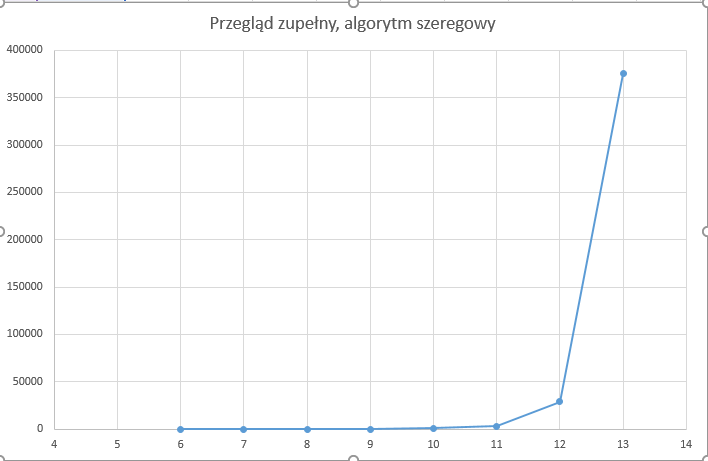
\includegraphics[width=0.7\linewidth]{bfS}
			\caption{Algorytm przeglądu zupełnego - szeregowo}
		\end{figure}
		\subsubsection{Czas działania algorytmu dla przeglądu zupełnego - wersja równoległa}
			Kolejnym krokiem było uruchomienie algorytmu przeglądu zupełnego na wielu wątkach. Dla każdego rozmiaru problemu został uruchomiony osobny wątek. Z racji charakteru tego rozwiązania niemożliwe jest badanie czasu dla osobnych problemów. Dlatego, zbadany czas jest wynikiem sumarycznym pracy algorytmu dla rozmiarów {\it 10, 11, 12}. Czas działania wyniósł {\it 29117ms}. 
			
			
		\subsubsection{Porównanie czasów wykonywania algorytmu przeglądu zupełnego} 
		Wykres przedstawiony poniżej pozwala zaobserwować różnice pomiędzy czasem wykonywania algorytmu zarówno dla metody szeregowej jak i równoległej.
			\begin{table}[H]
				\centering
				\caption{Porównanie czasu wykonywania algorytmów w wersji szeregowej i równoległej}
				\begin{tabular}{|c|c|}
					\hline Rodzaj algorytmu & czas działania [ms] \\ 
					\hline szeregowo & 32366 \\ 
					\hline równolegle& 29117 \\ 
							
					\hline 
				\end{tabular} 
			\end{table}	
			
		Poniżej przedstawiono wykres ukazujący różnicę w czasach działania algorytmu. Warto zauważyć, że czas algorytmu uruchomionego równolegle jest zbliżony do pojedynczego uruchomienia algorytmu dla przypadku szeregowego w rozmiarze 12 wierzchołków. Oznacza to, że w czasie jaki algorytm szeregowy potrzebuje na obliczenie jedynie problemu dla 12 wierzchołków, wersja równoległa zdołała obliczyć rozwiązanie dla rozmiaru 10 oraz 11. 
		\begin{figure}[H]
			\centering
			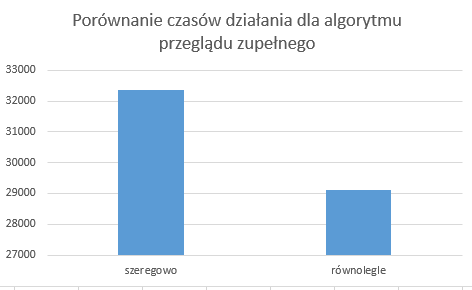
\includegraphics[width=0.7\linewidth]{bfSvsR.png}
			\caption{Przegląd zupełny-porównanie uruchomienia szeregowego i równoległego}
		\end{figure}
		
	\subsubsection{Czas działania algorytmu metodą podziału i ograniczeń  - wersja szeregowa}
		
		Czas działania algorytmu w tym przypadku jest dużo bardziej przystępny. W poniższym zestawieniu zebrane są testy czasów dla algorytmu uruchomionego sekwencyjnie, na jednym wątku. Charakterystyka algorytmu pozwala, a właściwie zmusza do badania algorytmu dla większych danych testowych.
	\begin{table}[H]
		\centering
		\caption{Uśrednione wyniki dla różnych ilości wierzchołków}
		\begin{tabular}{|c|c|}
			
			\hline Ilość miast  & czas działania algorytmu [ms] \\ 
			\hline  30& 35827 \\ 
			\hline  40& 73618 \\ 
			\hline  50& 95695\\ 
			\hline  60& 135795\\ 
			\hline 
		\end{tabular} 
	\end{table}
	
	Poniższy wykres przedstawia czas działania algorytmu dla metody podziału i ograniczeń. Jest to wykres zależności czasu działania algorytmu od ilość wierzchołków.

	\begin{figure}[H]
		\centering
		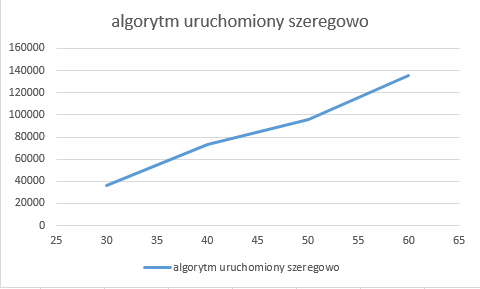
\includegraphics[width=0.9\linewidth]{bbS}
		\caption{ Czas działania algorytmu dla metody podziału i ograniczeń - wersja szeregowa }
	\end{figure}
	

	
	\subsubsection{Czas działania algorytmu metodą podziału i ograniczeń  - wersja równoległa}
	
	Podobnie jak w przypadku algorytmu przeglądu zupełnego tak i w tym przypadku charakterystyka sposobu wywoływania algorytmu nie pozwala na rozróżnienie czasu działania dla pojedynczych rozmiarów problemu. W tym przypadku algorytm został uruchomiony na kilku wątkach, po jednym dla każdego rozmiaru. Po zakończeniu działania wszystkich wątków został zmierzony czas. Sprawdzono czas działania algorytmu dla 30 i 40 wątków. Następnie dołożony został kolejny wątek liczący rozwiązanie dla 30, 40 i 50 wierzchołków.
		\\

		\begin{table}[H]
			\centering
			\caption{Wyniki działania równoległego algorytmu komiwojażera}
			\begin{tabular}{|c|c|}
				
				\hline Ilość miast  & czas działania algorytmu [ms] \\ 
				\hline  30,40 & 12925 \\ 
				\hline  30,40,50 & 188394 \\ 
				\hline 
			\end{tabular} 
		\end{table}
	
	 	
	\begin{figure}[H]
		\centering
		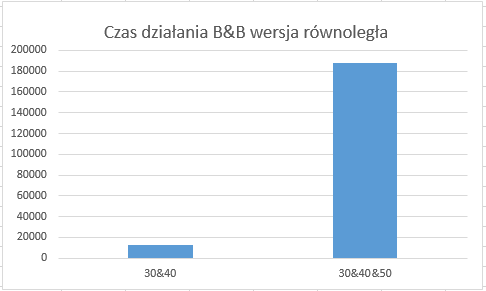
\includegraphics[width=0.9\linewidth]{bbR}
		\caption{ Czas działania algorytmu dla metody podziału i ograniczeń - wersja równoległa }
	\end{figure}
	


	\subsubsection{Porównanie czasu działania algorytmu metodą podziału i ograniczeń}
	Poniższy wykres przedstawia różnicę pomiędzy czasami wykonywania dla algorytmu podziału i ograniczeń. 
		
		\begin{figure}[H]
			\centering
			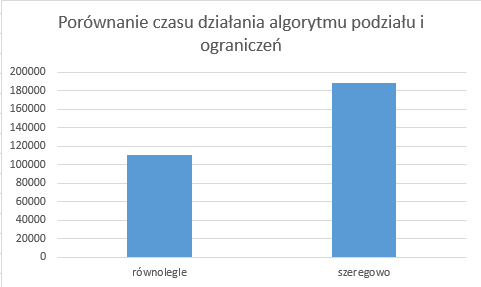
\includegraphics[width=0.9\linewidth]{bbRvsS}
			\caption{ Czas działania algorytmu dla metody podziału i ograniczeń porównanie czasów }
		\end{figure}
		
	\subsection{Czas wykonywania algorytmu przy stałym rozmiarze danych wejściowych i zmiennej liczbie wątków}	
		
		\subsubsection{Algorytm przeglądu zupełnego - działanie szeregowe}
	
			Podczas tych pomiarów uruchomiono algorytm dla stałego rozmiaru danych wejściowych. Zdecydowano się na macierz wejściową o rozmiarze 10 wierzchołków. \\
			W pierwszym kroku uruchomiono algorytm szeregowo, cztery razy. Wyniki poszczególnych przebiegów zebrano w poniżej tabeli:
			\begin{table}[H]
				\centering
				\caption{Czas działania algorytmu przeglądu zupełnego podczas pracy szeregowej}
				\begin{tabular}{|c|c|}
					
					\hline nr. przebiegu  & czas działania algorytmu [ms] \\ 
					\hline  1 & 271 \\ 
					\hline  2 & 258 \\ 
					\hline  3 & 248 \\ 
					\hline  4 & 245 \\ 
					\hline  5 & 247 \\ 
					\hline  6 & 233 \\ 
					\hline  7 & 310 \\ 
					\hline  8 & 262 \\ 
					\hline  9 & 243 \\ 
					\hline  10 & 321 \\ 
					\hline  suma & 2644 \\ 
					\hline 
				\end{tabular} 
			\end{table}
			
			Przeanalizowano zebrane dane i umieszczono na poniższym wykresie. Widać, że czasu są stałe, a pojedyncze odchyły są znikome.
			
				\begin{figure}[H]
					\centering
					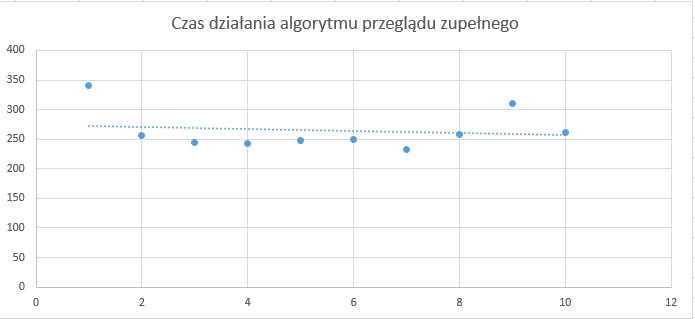
\includegraphics[width=0.9\linewidth]{BFS2}
					\caption{Czas działania algorytmu dla metody przeglądu zupełnego-uruchomienie szeregowe}
				\end{figure}
		\subsubsection{Algorytm przeglądu zupełnego - działanie równoległe}			
			Algorytm przeglądu zupełnego uruchomiony został dla tych samych danych. Do rozwiązywania problemów wykorzystano 10 wątków. Każdy uruchamiany był dla pojedynczej kopii instancji. \\
			
				\begin{table}[H]
					\centering
					\caption{Czas działania algorytmu przeglądu zupełnego podczas pracy równoległej}
					\begin{tabular}{|c|c|}
						
						\hline Czas działania:   & 598 ms\\ 
					
						\hline 
					\end{tabular} 
				\end{table}
		Z faktu charakteru działania algorytmów równoległych niemożliwe było wydzielenie czasów pojedynczych obliczeń. W związku z tym czas został zmierzony od uruchomienia do zakończenia działania wszystkich wątków.
		\subsubsection{Algorytm przeglądu zupełnego - porównanie czasów działania}	
			Warto zauważyć, że czas działania algorytmów uruchomionych równolegle jest dużo niższy, niż w przypadku działania szeregowego. W poniższej tabeli zebrano porównanie czasów dla algorytmu przeglądu zupełnego. Obydwa przypadki operowały na danych wejściowych w rozmiarze 10 wierzchołków, oraz zostały uruchomione dziesięciokrotnie.
			
				\begin{table}[H]
					\centering
					\caption{Porównanie czasów algorytmu przeglądu zupełnego}
					\begin{tabular}{|c|c|}
					\hline wersja równoległa:  & 598 ms\\ 	
					\hline wersja szeregowa:  & 2644 ms\\ 
					\hline 
					\end{tabular} 
				\end{table}	
				
			Poniżej przedstawiono dane w formie wykresu:
				\begin{figure}[H]
					\centering
					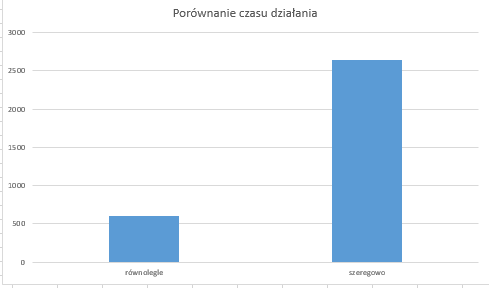
\includegraphics[width=0.9\linewidth]{bfRvsS}
					\caption{Porównanie czasów działania dla algorytmu przeglądu zupełnego}
				\end{figure}
				
			Z wykresów można wywnioskować, że przy rozmiarze problemu równym 10 czas działania algorytmu równoległego jest porównywalny z czasem uruchomienia algorytmu szeregowego trzy razy.
			
		\subsubsection{Algorytm podziału i ograniczeń - działanie szeregowe}
			Z racji szybkości obliczeń algorytmu podziału i ograniczeń, w porównaniu do algorytmu przeglądu zupełnego zwiększono rozmiar danych wejściowych do 50 wierzchołków. Podobnie jak w przypadku algorytmu uruchamianego szeregowo wykonano pomiar czasu dla 10 uruchomień algorytmu na tej samej instancji.
			\begin{table}[H]
				\centering
				\caption{Czas działania algorytmu przeglądu zupełnego podczas pracy szeregowej}
				\begin{tabular}{|c|c|}
					
					\hline nr. przebiegu  & czas działania algorytmu [ms] \\ 
					\hline  1 & 6358 \\ 
					\hline  2 & 2060 \\ 
					\hline  3 & 1560 \\ 
					\hline  4 & 2654 \\ 
					\hline  5 & 2777 \\ 
					\hline  6 & 2803 \\ 
					\hline  7 & 2943 \\ 
					\hline  8 & 2595 \\ 
					\hline  9 & 1749 \\ 
					\hline  10 & 2727 \\ 
					\hline  suma & 28226 \\ 
					\hline 
				\end{tabular} 
			\end{table}
	
		\begin{figure}[H]
			\centering
			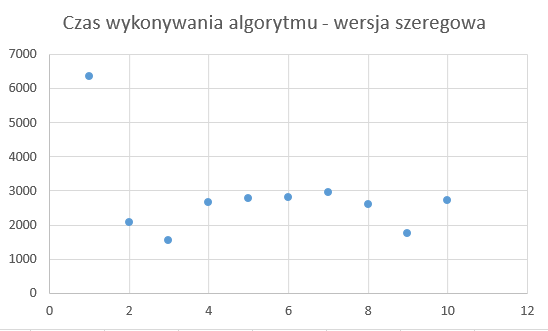
\includegraphics[width=0.9\linewidth]{bbS2}
			\caption{Czas wykonywania algorytmu - wersja szeregowa}
		\end{figure}
	
	
		\subsubsection{Algorytm podziału i ograniczeń - działanie równoległe}
			Badanie algorytmu podziału i ograniczeń w wersji równoległej nie było łatwe, ponieważ dla założonych danych ilość pamięci potrzebnej do obliczeń wymagała zmiany ustawień uruchomienia programu, tak aby dostał on więcej zasobów pamięci. Po tej zmianie czas przetwarzania dla 50 wierzchołków wyniósł : \textit{26749 ms}. Badany czas dotyczy 10 wątków uruchomionych jednocześnie dla jednakowej instancji macierzy o rozmiarze 50 wierzchołków.
			
		\subsubsection{Algorytm podziału i ograniczeń - porównanie czasu działania}
			
				\begin{table}[H]
					\centering
					\caption{Czas działania algorytmu przeglądu zupełnego porównanie}
					\begin{tabular}{|c|c|}
						
						\hline rodzaj wersji& czas działania algorytmu [ms] \\ 
						\hline równoległa  & 26749 \\ 
						\hline szeregowa   & 28226 \\ 
						\hline 
					\end{tabular} 
				\end{table}
	
	Czas wykonywania algorytmu zrównoleglonego jest lepszy od czasu wykonywania szeregowego. W odróżnieniu od poprzedniego algorytmu różnica między czasami nie jest taka znaczna. Może to być spowodowane duża ilością pamięci potrzebną podczas pracy algorytmu podziału i ograniczeń. 
	
	
	\subsection{Analiza i ocena jakości}
		Przeanalizowanie jakości jest zadaniem nietrywialnym, lecz możliwym. Algorytm przeglądu zupełnego daje rozwiązanie optymalne zawsze. Kosztowne jest jednak sprawdzenie wszystkich możliwych rozwiązań. W wykresów przestawionych w tym dokumencie można z łatwością wywnioskować, że czas działania rośnie w sposób wykładniczy. Przy 15 wierzchołkach problem jest praktycznie nierozwiązywalny przez domowe komputery. Drugie podejście analizowanie w tym projekcie pozwala na znaczne zredukowanie czasu działania. Jednakże odbywa się to kosztem pamięci. Jest to spowodowane faktem przechowywania w pamięci drzewa przeszukiwań, które podczas pracy algorytmu rozrasta się bardzo szybko. Podczas badań czasu pracy algorytmu Java zwróciła błąd przepełnienia pamięci już dla 75 wierzchołków. Nie jest to wartość deterministyczna, ponieważ zależy od wygenerowanych danych wejściowych. Może okazać się, ze szybko znajdziemy minimum lokalne funkcji drogi i odrzucone zostaną rozwiązania na pewno nie optymalne.
	\subsection{Wnioski z testów i badań}
		Największą trudnością podczas badań było wstępne oszacowanie czasu pracy algorytmów. Jeżeli rozmiar problemu wejściowego był zbyt duży, czas oczekiwania na wyniki stawał się zbyt duże.
		
\section{Podsumowanie}
	Wykonanie projektu pozwoliło uzmysłowić nam istotę dobrego planowania pracy podczas operacji na wielu wątkach. Najistotniejszymi problemami jest synchronizowany dostęp do zasobów podczas pracy wielu wątków. Zmierzyliśmy się z tym problem podczas mierzenia czasu pracy algorytmów. Zastosowanie odpowiednich technik i badań operacyjnych umożliwiło implementację algorytmów. Algorytmy rozwiązujące optymalizacyjny problem komiwojażera są tematem rozległym i nietrywialnym.
\section{Literatura}
[1] Thomas Cormen, \emph{Wstęp do algorytmów}, Leiserson, Rivest, Stein 7nd edition, 2005. \newline [2] John Little, \emph{An algorithm for the traveling salesman problem}, Little, John 1963.







\end{document}\documentclass{article}
